\documentclass[17pt]{beamer} %Makes presentation
%\documentclass[handout]{beamer} %Makes Handouts
\usetheme{Singapore} %Gray with fade at top
\useoutertheme[subsection=false]{miniframes} %Supppress subsection in header
\useinnertheme{rectangles} %Itemize/Enumerate boxes
\usecolortheme{seagull} %Color theme
\usecolortheme{rose} %Inner color theme

\definecolor{light-gray}{gray}{0.75}
\definecolor{dark-gray}{gray}{0.55}
\setbeamercolor{item}{fg=light-gray}
\setbeamercolor{enumerate item}{fg=dark-gray}

\setbeamertemplate{navigation symbols}{}
%\setbeamertemplate{mini frames}[default]
%\setbeamercovered{dynamics}
\setbeamerfont*{title}{size=\Large,series=\bfseries}
\setbeamerfont{footnote}{size=\tiny}

%\setbeameroption{notes on second screen} %Dual-Screen Notes
%\setbeameroption{show only notes} %Notes Output

\setbeamertemplate{frametitle}{\vspace{.5em}\bfseries\insertframetitle}
\newcommand{\heading}[1]{\noindent \textbf{#1}\\ \vspace{1em}}

\usepackage{bbding,color,multirow,times,ccaption,tabularx,graphicx,verbatim,booktabs}
\usepackage{colortbl} %Table overlays
\usepackage[english]{babel}
%\usepackage[latin1]{inputenc}
%\usepackage[T1]{fontenc}
\usepackage{lmodern}

%\author[]{Thomas J. Leeper}
\institute[]{
  \inst{}%
  Department of Government\\London School of Economics and Political Science
}

\usepackage{tikz}
\usetikzlibrary{shapes,arrows,decorations.pathreplacing,calc}

\title{Ethics and Research Integrity}

\date[]{}

\begin{document}

\frame{\titlepage}

\frame{\tableofcontents}

\section{Ethics}
\frame{\tableofcontents[currentsection]}

\frame{
\frametitle{History: Key Moments}

\small

\begin{enumerate}
\item Tuskegee (1932-1972) and Guatemala (1946-1948) Studies
\item Nuremberg Code (1947)
\item Helsinki Declaration (1964)
\item U.S. 45 CFR 46 (1974) and ``Common Rule'' (1991)
\item The Belmont Report (1979)
\item EU Data Protection Directive (1995; 2012)
	\begin{itemize}
	\item UK Data Protection Act (1998)
	\end{itemize}
\end{enumerate}
}


\frame{
	\frametitle{Helsinki Declaration}
	
	\small
	\begin{itemize}
	\item Adopted by the World Medical Association in 1964\footnote{\url{http://www.bmj.com/content/2/5402/177}}
	\item Narrowly focused on medical research
	\item Expanded the Nuremberg Code
		\begin{itemize}
		\item Relaxed consent requirements
		\item Risks should not exceed benefits
		\item Institutionalization of ethics oversight
		\end{itemize}
	\item<2-> Do these rules apply to non-experimental research? To non-medical research?
	\end{itemize}

}

\frame{
	\frametitle{Social Science Examples}
	\begin{enumerate}\itemsep2em
	\item \href{https://www.youtube.com/watch?v=yr5cjyokVUs}{Milgram Obedience Study (1961)}
	\item \href{https://www.youtube.com/watch?v=760lwYmpXbc}{Stanford Prison Study (1971)}
	\end{enumerate}
}


\frame{
	\frametitle{The Belmont Report}
	
	\small
	\begin{itemize}
	\item Commissioned by the U.S. Government in 1979\footnote{\url{http://www.hhs.gov/ohrp/humansubjects/guidance/belmont.html}}
	\item Three overarching principles:
		\begin{enumerate}
		\item Respect for persons
		\item Beneficence
		\item Justice
		\end{enumerate}
	\item Three policy implications:
		\begin{itemize}
		\item Informed consent
		\item Assessment of risks/benefits
		\item Care for vulnerable populations
		\end{itemize}
	\end{itemize}

}


\frame{
	\frametitle{Informed Consent}
	\begin{itemize}
	\item Persons must consent to being a research subject
	\item<2-> What this means in practice is complicated
		\begin{itemize}
		\item What is research?
		\item What is consent?
		\item What is ``informed'' consent?
		\end{itemize}
	\item<3-> Cross-national variations
		\begin{itemize}
		\item Consent forms required in U.S.
		\item Not required in UK
		\end{itemize}
	\end{itemize}

}

\frame{
\frametitle{Benefits and Harm}
	\begin{itemize}\itemsep2em
	\item What is a ``benefit''?
	\item What is a ``harm''?
	\item How do we balance the two?
	\end{itemize}
}


\frame{
	\frametitle{Privacy}
	\begin{itemize}
	\item EU Data Protection Directive (1995) and UK Data Protection Act (1998)
	\item Deals with ``personal data''
	\item Data can be processed when:
		\begin{itemize}
		\item Consent is given
		\item Data are used for a ``legitimate'' purpose
		\item Anonymous or confidential
		\end{itemize}
	\item Data cannot leave the EU except under conditions
	\end{itemize}
}


\frame{
	\frametitle{{\normalsize Lots of Other Ethical Questions}}
	\begin{enumerate}
	\item<2-> Funding
	\item<3-> Independence and Politicization
	\item<4-> Vulnerable populations (e.g. children, sick)
	\item<5-> Cross-national research
	\item<6-> Participant-observation disclosures
	\item<7-> End uses/users of research
	\item<8-> Others?
	\end{enumerate}
}


\frame{

\Large 

\begin{center}
Questions?
\end{center}

}


\frame{

\frametitle{Activity!}

\begin{itemize}\itemsep1em
\item Read each ethical scenarios
\item Decide what ethical issues are raised by the scenario (if any)
\item Decide what modifications are necessary for the project to be ethically acceptable
\end{itemize}

}




\frame{}

\section{Ethics at LSE}
\frame{\tableofcontents[currentsection]}


\frame{
\frametitle{Research Ethics at LSE}

\begin{itemize}
\item Ethics Code \footnote{\url{http://www.lse.ac.uk/intranet/LSEServices/ethics/home.aspx}}
\item Research Ethics Policy \footnote{\url{http://www.lse.ac.uk/intranet/LSEServices/policies/pdfs/school/resEthPolPro.pdf}}
\item Levels of review:
	\begin{enumerate}
	\item Staff: Self-certification
	\item Students: Supervisor certification
	\item LSE Research Ethics Committee
	\item External review
	\end{enumerate}
\end{itemize}

}


\frame{

\begin{center}
\href{http://www.lse.ac.uk/intranet/researchAndDevelopment/researchDivision/policyAndEthics/ethics-annexC.pdf}{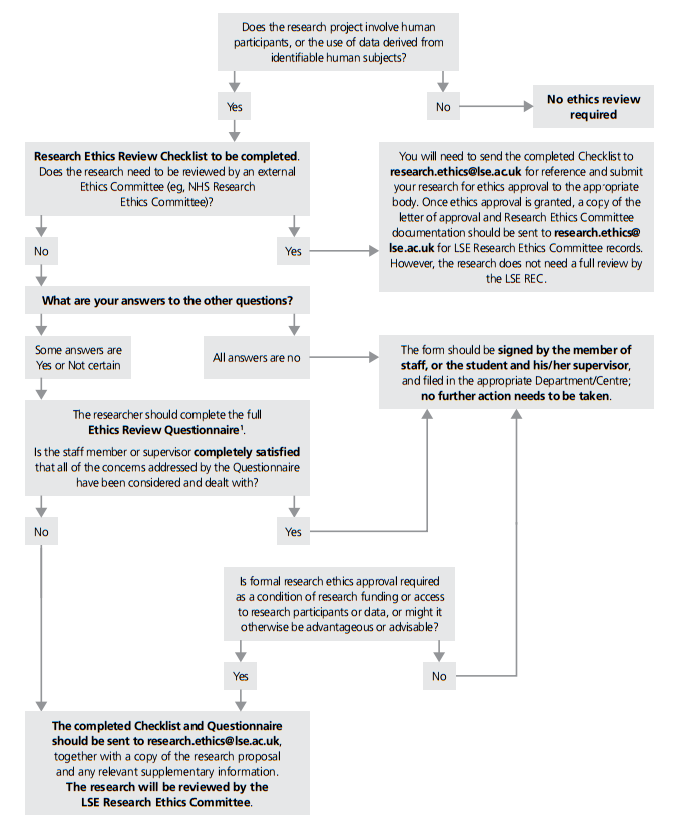
\includegraphics[width=\textwidth]{images/lse_ethics_flowchart}}
\end{center}

}

\frame{
\frametitle{Activity!}

\begin{itemize}
\item Complete an LSE Ethics form for your proposed research project
\end{itemize}

}


\appendix
\frame{}

\end{document}
